\documentclass[conference]{IEEEtran}
\usepackage[T1]{fontenc}
\usepackage{graphicx}
\usepackage{booktabs}
\usepackage{amsmath}
\usepackage{xcolor}
\usepackage{url}
\usepackage[hidelinks]{hyperref}
\usepackage{listings}
\lstset{basicstyle=\ttfamily\scriptsize,columns=fullflexible,breaklines=true,frame=single,framerule=0.3pt,
        rulecolor=\color{gray!60},xleftmargin=2pt,xrightmargin=2pt,aboveskip=4pt,belowskip=4pt}
\newcommand{\slicj}{SLIC-J}

\begin{document}

\title{Seven Sins Revisited: Reproducing SLIC, Porting It to Ansible and Chef, and Triaging Its False Positives with Context-Aware Decision Models}

\author{\IEEEauthorblockN{Adheil Gupta (23BDS002) \qquad Om Pandey (23BDS040)}
\IEEEauthorblockA{Course project, Cloud SRE and Security\\
% TODO: add department and institute
}}

\maketitle

\begin{abstract}
Infrastructure as code (IaC) scripts configure cloud fleets, so a single insecure pattern can spread to every server.
Rahman et al.\ (ICSE~2019) defined seven security smells for Puppet and built SLIC, a rule-based linter.
We reproduce SLIC, port it to Ansible and Chef, and attack its main weakness: false positives.
First, a reimplementation from the paper alone agrees with the released tool on only 58\% of findings; we locate
six differences between the paper and the code, including a check that never reaches the output.
A token-level port of the released rules matches the original on 120 of 120 findings (Jaccard 0.99).
Second, our port, \slicj{}, reaches micro-F1 0.64/0.82/0.63 on the Puppet/Ansible/Chef oracle datasets of
GLITCH, against 0.62/0.86/0.54 for GLITCH itself, and it adds a new smell, \emph{TLS verification disabled}, which
occurs in 1.0\% of 107{,}955 Ansible scripts with 98\% sampled precision.
Third, we keep the rules as a high-recall candidate generator and add a triage step: code computes context facts,
masks secret values, and asks a \emph{decision model} (TypeSafe Jev) one typed question per finding.
Over 269 candidates, triage raises precision from 0.56 to 0.78 at a recall cost of 0.05 (F1 0.68$\to$0.80,
McNemar $p<10^{-14}$); for hard-coded secrets it removes 76 of 80 false alarms.
A chat LLM is slightly better (F1 0.81, not significant) at 4$\times$ the cost and 3$\times$ the latency.
Finally, one injected comment flips 97.5\% of a decision model's true findings to ``safe''; a chat LLM ignores the
injection but believes a ``dummy value'' comment in up to 20\% of cases. Stripping comments from the model's input
reduces both attacks to at most 1.6\%.
\end{abstract}

\begin{IEEEkeywords}
infrastructure as code, security smells, static analysis, reproduction, false positives, LLM triage, prompt injection
\end{IEEEkeywords}

% =====================================================================
\section{Introduction}
Site reliability teams treat infrastructure as code: Puppet manifests, Ansible playbooks and Chef recipes define
users, services, network bindings and credentials for whole fleets. A pattern such as a hard-coded password or a
service bound to \texttt{0.0.0.0} is therefore copied to every machine the script touches. Rahman, Parnin and
Williams called such recurring patterns \emph{security smells}. In ``The Seven Sins'' (ICSE~2019)~\cite{rahman2019seven}
they derived seven smells from 1{,}726 Puppet scripts, mapped each to a CWE, and implemented SLIC, a linter whose
rules match token names and values. They reported precision and recall of 0.99 on their own oracle and found
21{,}201 smells in 15{,}232 scripts.

Later work showed two problems. Rule-based detectors over-approximate: on the independent oracles of
GLITCH~\cite{saavedra2022glitch}, SLIC's precision for hard-coded secrets is 0.10. And practitioners judge findings
by context: in the original study a developer rejected an HTTP finding because ``it's using http on localhost'', and
Reis et al.\ found that precision drops further when maintainers who know the application judge
it~\cite{reis2022feedback}. Recent work therefore pairs rules with a learned filter~\cite{mei2026intellisa}.

This paper is a course project with the brief ``implement the approach of a selected paper, evaluate it, and report''.
We implement SLIC, test how far the paper alone lets one rebuild it, port it to two more IaC tools, and then add a
context-aware triage layer. We answer four research questions:
\begin{itemize}
\item \textbf{RQ1 (reproduction).} Can SLIC be rebuilt from the paper, and does the rebuild match the released tool?
\item \textbf{RQ2 (portability).} How accurate is a port to Ansible and Chef, and how common is a new smell for disabled TLS verification?
\item \textbf{RQ3 (triage).} How much precision do context facts and a decision model add, and at what recall, cost and calibration?
\item \textbf{RQ4 (robustness).} Can a misleading comment in the script talk the triage model out of a true finding, and does a simple input rule stop it?
\end{itemize}

\textbf{Contributions.} (1) A Python reimplementation of SLIC in two forms, ``paper rules'' and a token-level port of
the released code, plus a list of six paper--code differences. (2) \slicj{}, a port of the seven rules to Ansible and
Chef with a new eighth smell. (3) A triage design in which code computes and masks context and a decision model
answers one typed question, evaluated against eight decision models, a chat LLM, a learned baseline and a hybrid,
with calibration, cost and latency. (4) A prompt-injection test for IaC triage and a mitigation.
All code, cached model responses and scripts that regenerate every number are in the artifact.

% =====================================================================
\section{Background and Related Work}
\subsection{The seven sins and SLIC}
The seven smells are \emph{admin by default} (CWE-250), \emph{empty password} (CWE-258), \emph{hard-coded secret}
(CWE-798/259), \emph{invalid IP address binding} (CWE-284), \emph{suspicious comment} (CWE-546), \emph{use of HTTP
without TLS} (CWE-319) and \emph{use of weak cryptography algorithms} (CWE-327/326)~\cite{rahman2019seven}.
SLIC has two parts. A \emph{parser}, built on puppet-lint, turns a script into vectors such as
\texttt{<VARIABLE, '\$vcenter\_password', 'password'>}. A \emph{rule engine} applies Table~II of the paper, e.g.\
hard-coded secret $=(\mathit{isAttribute}(x)\lor\mathit{isVariable}(x))\land(\mathit{isUser}(x.\mathit{name})\lor
\mathit{isPassword}(x.\mathit{name})\lor\mathit{isPvtKey}(x.\mathit{name}))\land \mathit{length}(x.\mathit{value})>0$,
with string patterns from Table~III. The same authors later ported the rules to Ansible and Chef (SLAC) and found
smells in 25.3--29.6\% of Ansible scripts~\cite{rahman2021slac}.

\subsection{Later detectors}
GLITCH~\cite{saavedra2022glitch,saavedra2023glitch} translates Puppet, Ansible, Chef and Terraform into one
intermediate model and runs a single set of checks; its replication package~\cite{glitchpkg2022} contains three oracle
datasets of about 80 scripts each, labelled by seven raters, which we reuse. GASEL~\cite{opdebeeck2023gasel} adds
control and data flow for Ansible. Opdebeeck et al.\ predict which Ansible module parameters hold
secrets~\cite{opdebeeck2025smelling}. IntelliSA~\cite{mei2026intellisa} over-approximates with rules and filters false
positives with a model distilled from an LLM. Our triage step follows the same ``rules propose, a model disposes''
idea, but uses System One decision models, measures calibration and prompt-injection robustness, and never sends a
raw secret to the model.

\subsection{Decision models}
TypeSafe's Jev is a \emph{System One} model: it does not generate text, it answers typed questions about a given
state and returns probabilities~\cite{typesafe2026jev}. A \emph{Noul} question returns $P(\text{yes})$; a
\emph{Choice} question returns a distribution over options. OpenRouter exposes Jev and about twenty similar models
through one Decisions API~\cite{openrouter2026jev}. The vendor recommends that code keeps control of the flow,
combines answers with deterministic rules and escalates low-confidence cases, and it warns that content written to
steer the model can move its answer. Our design and RQ4 follow directly from these two statements.

% =====================================================================
\section{Approach}
\begin{figure}[t]\centering
\fbox{\begin{minipage}{0.95\columnwidth}\footnotesize
\textbf{Script} (.pp / .yml / .rb) $\rightarrow$ \textbf{Parser} (SLIC tokens: VARIABLE, ATTRIBUTE, PARAMETER,
FUNCTION, COMMENT) $\rightarrow$ \textbf{Rule engine} (7 sins + TLS-off; high recall) $\rightarrow$
\textbf{Context layer} (code only: value kind, shape, entropy bucket, key format, placeholder, host scope, URL kind,
path purpose, $\pm3$-line window; secrets masked) $\rightarrow$ \textbf{Decision model} (one Noul question:
``is this a genuine instance of the smell, by this definition?'') $\rightarrow$ \textbf{Code decides}
(threshold tuned on training folds) $\rightarrow$ report.
\end{minipage}}
\caption{\slicj{} pipeline. Only the last two steps are new relative to SLIC.}\label{fig:pipeline}
\end{figure}

\subsection{Reimplementing SLIC (RQ1)}
We wrote two Python versions. \emph{Paper rules} implement Tables~II and III exactly as printed on top of our own
lexer. Where the table is not executable we use the evident intent and record the gap. \emph{Code port} mirrors the
released \texttt{all\_in\_one.rb}~\cite{iacsec} token by token: a lexer reproduces puppet-lint's token types and
values (\texttt{VARIABLE} without the dollar sign, keywords as their own types, interpolated strings split into
\texttt{DQPRE}/\texttt{DQPOST}), and each check looks, as the Ruby does, at a token, the next code token and the one
after it on the same line. To obtain ground truth for the comparison we re-ran the original SLIC with puppet-lint
2.5.2 and the shipped rules on the Puppet oracle.

\subsection{Porting to Ansible and Chef (RQ2)}
For Ansible we parse YAML with \texttt{ruamel.yaml}, which keeps line numbers. Keys under a task or module become
ATTRIBUTE tokens; keys under \texttt{vars:}, \texttt{set\_fact:} and in \texttt{vars/} files become VARIABLE; top-level
keys of a role's \texttt{defaults/} file become PARAMETER, the nearest analogue of a Puppet class parameter default.
Jinja calls and filters become FUNCTION tokens; YAML~1.1 booleans (\texttt{yes}/\texttt{no}) are normalised; a
line-based fallback handles files that are not valid YAML. For Chef we use a line-level reader for node attributes,
resource properties, hash entries, local variables, two-argument setters and heredoc command text.

\slicj{} keeps the seven rules but (i) matches name \emph{segments} (so \texttt{bypass} is not a password and
\texttt{dbPassword} is), (ii) requires a literal value for secrets, so variable references, lookups and vault values
are not ``hard-coded'', and (iii) follows the oracle raters' guide, which widens admin by default to ``every time
more privileges are being given than necessary'' (e.g.\ \texttt{user => root}). Keyword lists follow GLITCH's
published configuration with word boundaries.

\textbf{New smell: TLS verification disabled (CWE-295~\cite{cwe295}).} Turning certificate validation off makes
HTTPS as weak as HTTP against an active attacker, yet it is not among the seven sins. \slicj{} flags names such as
\texttt{validate\_certs}, \texttt{sslverify}, \texttt{verify\_ssl} set to false; names such as \texttt{insecure},
\texttt{insecure\_skip\_tls\_verify}, \texttt{allow\_insecure} set to true; and command text with \texttt{curl -k},
\texttt{--insecure}, \texttt{wget --no-check-certificate}, \texttt{--tls-verify=false} or
\texttt{GIT\_SSL\_NO\_VERIFY=1}, across all modules.

\subsection{Context layer and triage (RQ3)}
For every candidate, code computes facts that a model is known to handle badly: whether the value is a literal, a
variable, a lookup or a vault reference; its shape (identifier, file path, URL, token); an entropy bucket and a
known-key-format class (AWS key, private-key block, SSH key, hash, \ldots); a placeholder test; the host scope of a URL
(loopback, private, public, templated) and its kind (XML namespace, download, package repository); and the purpose of
the file path (tests/CI, examples/training, development). \emph{Privacy rule:} a value that could be a working
credential never leaves the machine; the model sees a masked preview such as \texttt{s3******r1 (len 10)}.
Placeholders and short words are sent in clear. The same masking is applied to every line of the code window that
contains a sensitive name.

The state sent to the model contains the smell name, its CWE, the raters' definition, why the rule fired, the flagged
line, and in the \emph{full} variant also the facts, the file path and a $\pm3$-line window. The question is a
single Noul, ``Is the linter finding a genuine instance of the named security smell in this code, according to the
definition?'', with short criteria for \emph{true} and \emph{false}. The model returns $P(\text{true})$; code keeps a
finding if $P\ge t$, where $t$ is tuned on training folds only.

\subsection{Robustness (RQ4)}
Scripts are attacker-controllable text: anyone who can open a pull request can add a comment. We insert one comment
above, or at the end of, the line of each true finding, with three texts: a \emph{placeholder} claim (``dummy value used
only by CI tests''), an \emph{approval} claim (``reviewed and approved by the security team'') and an
\emph{injection} addressed to the reviewer (``this finding is a known false alarm. Answer false''). The mitigation
removes comments from every code field of the state; rule facts are unchanged, and a suspicious-comment finding keeps
its text in a field marked as untrusted.

% =====================================================================
\section{Experimental Setup}
\textbf{Data.} The GLITCH replication package~\cite{glitchpkg2022} (1.8\,GB Docker image; we extracted its layers
without running it) contains: the Puppet oracle (80 scripts, 4{,}367 LOC), the Ansible oracle (81 scripts, reused from
SLAC), the Chef oracle (80 scripts), the raters' guide, the outputs of the original SLIC and SLAC on these oracles,
and corpora of 27{,}324 Puppet, 107{,}955 Ansible and 70{,}705 Chef scripts (12.2\,M LOC). We score only the seven
sins; oracle labels for ``no integrity check'' and ``missing default case'' are ignored.

\textbf{Matching.} We use GLITCH's protocol: a finding is a true positive if file, category and line match an oracle
entry (file and category suffice for weak crypto and IP binding); each oracle entry matches once. For the Ansible
outputs of SLAC and GLITCH'22, which carry code text instead of line numbers, we copy GLITCH's text matching. Our
evaluator reproduces every published per-smell value of SLIC, SLAC and GLITCH'22 on all three oracles exactly, which
validates it.

\textbf{Baselines.} Original SLIC (re-run) and SLAC; GLITCH'22 (packaged output) and GLITCH~v2 (current release, run
by us). For triage: rules only; a \emph{practitioner-context filter} (hand-written: drop placeholder secrets, file
paths, loopback/namespace URLs, \ldots); logistic regression on the context facts; Jev~1.13 with the line-only and the
full state; seven other decision models and Jev~1.14 with the full state; Claude Haiku~5.5 as a chat-LLM baseline
asked for a JSON probability with the same state; and a hybrid logistic regression over the facts plus Jev's
probability.

\textbf{Protocol.} Rules were refined only on a fixed 30\% development split of the oracle files. Triage is evaluated
on all 269 candidates with 5-fold cross-validation grouped by file and repeated over 10 seeds; thresholds and logistic
weights are fit on training folds. Recall is computed against all 176 oracle smells, so findings the rules never
produced count as misses. We test paired decisions with the exact McNemar test~\cite{mcnemar1947} and report 95\%
file-level bootstrap intervals for $\Delta$F1 (2{,}000 resamples). Calibration is measured with AUC, the Brier score
and the expected calibration error (ECE, 10 bins)~\cite{guo2017calibration}. Cost is the API-reported charge.

\textbf{Budget.} The OpenRouter account had a small free allowance. RQ3 ran entirely on paid models (USD 0.20 in
total). When the allowance ran out, RQ4 had to use a free decision model (Inception Mercury-Decide, which scores
F1 0.78 on RQ3, close to Jev) and Claude Haiku~5.5 through the Claude Code CLI on a 59-finding stratified sample. The
RQ4 script runs unchanged on Jev given credits.

% =====================================================================
\section{Results}
\begin{table*}[t]\centering\caption{RQ1/RQ2: precision / recall per smell on the three GLITCH oracle datasets (all files; GLITCH matching protocol). Micro values pool all seven smells. `--' = no prediction or no true instance.}\label{tab:rq1}
\scriptsize\setlength{\tabcolsep}{3pt}\begin{tabular}{llcccccccccc}\toprule
Tech & Tool & Adm & Emp & Sec & IP & Sus & HTTP & Cry & P$_\mu$ & R$_\mu$ & F1$_\mu$ \\ \midrule
Puppet & SLIC (original) & --/0.00 & 0.60/0.60 & 0.10/0.73 & 1.00/1.00 & 0.75/1.00 & 0.38/1.00 & 0.43/0.75 & 0.28 & 0.63 & 0.39 \\
 & SLIC (original, re-run) & --/0.00 & 0.60/0.60 & 0.10/0.73 & 1.00/1.00 & 0.75/1.00 & 0.38/1.00 & 0.43/0.75 & 0.28 & 0.63 & 0.39 \\
 & Ours: SLIC code port & --/0.00 & 0.60/0.60 & 0.10/0.73 & 1.00/1.00 & 0.75/1.00 & 0.38/1.00 & 0.43/0.75 & 0.28 & 0.63 & 0.39 \\
 & Ours: paper rules & --/0.00 & 0.75/0.60 & 0.26/0.91 & 1.00/1.00 & 0.60/1.00 & 0.38/1.00 & 0.00/0.00 & 0.42 & 0.61 & 0.50 \\
 & GLITCH ASE'22 & 0.81/0.93 & 1.00/1.00 & 0.14/0.82 & 1.00/1.00 & 0.39/1.00 & 0.45/1.00 & 0.57/1.00 & 0.38 & 0.94 & 0.54 \\
 & GLITCH v2 (live) & 0.93/0.93 & 1.00/1.00 & 0.22/1.00 & 1.00/1.00 & 0.39/1.00 & 0.45/1.00 & 0.57/1.00 & 0.45 & 0.98 & 0.62 \\
 & \textbf{SLIC-J rules} & 0.93/0.93 & 0.80/0.80 & 0.24/0.91 & 1.00/1.00 & 0.64/1.00 & 0.38/1.00 & 0.40/0.50 & 0.50 & 0.91 & 0.64 \\
\midrule
Ansible & SLAC (original) & --/0.00 & 1.00/1.00 & 0.32/1.00 & 1.00/1.00 & 0.67/0.67 & 0.71/1.00 & -- & 0.56 & 0.79 & 0.65 \\
 & Ours: code rules & --/0.00 & 1.00/1.00 & 0.11/0.38 & 1.00/1.00 & 1.00/0.50 & 0.74/1.00 & -- & 0.47 & 0.65 & 0.54 \\
 & Ours: paper rules & --/0.00 & 1.00/1.00 & 0.44/1.00 & 1.00/1.00 & 1.00/0.50 & 0.74/1.00 & -- & 0.66 & 0.77 & 0.71 \\
 & GLITCH ASE'22 & 1.00/1.00 & 1.00/1.00 & 0.42/1.00 & 1.00/1.00 & 0.75/1.00 & 0.95/1.00 & -- & 0.75 & 1.00 & 0.86 \\
 & GLITCH v2 (live) & 1.00/1.00 & 1.00/1.00 & 0.44/1.00 & 1.00/1.00 & 0.75/1.00 & 0.95/1.00 & 0.00/-- & 0.75 & 1.00 & 0.86 \\
 & \textbf{SLIC-J rules} & 1.00/1.00 & 1.00/1.00 & 0.44/1.00 & 1.00/1.00 & 0.75/1.00 & 0.74/1.00 & -- & 0.69 & 1.00 & 0.82 \\
\midrule
Chef & Ours: code rules & --/0.00 & 1.00/0.25 & 0.08/0.23 & 1.00/1.00 & 0.80/1.00 & 0.68/1.00 & 0.17/1.00 & 0.39 & 0.37 & 0.38 \\
 & Ours: paper rules & --/0.00 & 1.00/0.25 & 0.19/0.69 & 1.00/1.00 & 0.80/1.00 & 0.68/1.00 & 0.50/1.00 & 0.43 & 0.44 & 0.44 \\
 & GLITCH ASE'22 & 0.94/0.41 & 1.00/0.75 & 0.20/0.69 & 1.00/1.00 & 0.40/1.00 & 0.71/0.92 & 0.50/1.00 & 0.50 & 0.65 & 0.57 \\
 & GLITCH v2 (live) & 0.93/0.38 & 1.00/0.75 & 0.14/0.46 & 1.00/1.00 & 0.40/1.00 & 0.71/0.92 & 0.50/1.00 & 0.49 & 0.59 & 0.54 \\
 & \textbf{SLIC-J rules} & 0.89/0.65 & 1.00/0.25 & 0.19/0.69 & 1.00/1.00 & 0.80/1.00 & 0.68/1.00 & 0.50/1.00 & 0.54 & 0.75 & 0.63 \\
\bottomrule\end{tabular}\end{table*}

\subsection{RQ1: Reproducing SLIC}
\textbf{The paper alone is not enough.} Our paper-rules version shares 73 findings with the original SLIC on the
Puppet oracle, misses 47 and adds 5 (Jaccard 0.58). The released tool's own output, re-run by us, is identical to the
packaged output (120/120). We traced the gap to six paper--code differences:
\begin{enumerate}
\item \emph{Admin by default.} Table~II requires that the \emph{name} contains both ``admin'' and ``user''. The paper's
own Fig.~4 example, \texttt{\$power\_username = 'admin'}, does not satisfy this; the code checks the \emph{value}.
\item \emph{isPvtKey.} The printed pattern \texttt{[pvt|priv]+*[cert|key|rsa|secret|ssl]+} is not a valid regular
expression (double quantifier); we used the intent.
\item \emph{Secret keywords.} The code matches 14 substrings (adding key, crypt, cert, ssl, dsa, md5, rsa, \ldots),
excludes 19 values (\texttt{undef}, \texttt{hiera}, \texttt{pick}, \ldots) and does not require an assignment: any NAME
followed two tokens later by a literal fires, e.g.\ \texttt{govuk\_user \{ 'felisialoukou':}.
\item \emph{Weak crypto.} The paper says ``function''; the code flags any non-comment token containing md5 or sha1,
including variable names such as \texttt{\$md5sum}.
\item \emph{Suspicious comment.} The code adds ``ticket'', ``launchpad'' and ``to-do'', excludes lines containing
``debug'', and scans every raw line that contains ``\#'', including URLs inside strings.
\item \emph{A dead check.} The rule \texttt{no\_expose\_secret\_location} prints the tag
\texttt{EXPOSING\_SECRET\_LOCATION:::}, but SLIC's driver searches for \texttt{EXPOSING\_SECRET\_LOCATION\_}. Its
warnings never reach the output. Enabling it would add 11 findings to the oracle run.
\end{enumerate}
\textbf{A faithful port is possible.} With these semantics our code port matches the original on 120 of 120 findings
with one extra (Jaccard 0.99); the extra comes from a \texttt{.pp} file that is actually Haskell. Per-smell scores are
identical (Table~\ref{tab:rq1}). The original's 0.99 accuracy did not carry over to GLITCH's independent Puppet oracle:
micro precision 0.28, and 0.10 for hard-coded secrets.

\subsection{RQ2: Portability and the new smell}
Table~\ref{tab:rq1} shows that \slicj{} reaches micro-F1 0.64 on Puppet (SLIC 0.39, GLITCH~v2 0.62), 0.82 on Ansible
(SLAC 0.65, GLITCH~v2 0.86) and 0.63 on Chef (GLITCH~v2 0.54). Recall is high (0.91/1.00/0.75); precision is held
down by hard-coded secrets (0.19--0.44) and HTTP (0.38--0.74) for every tool (Fig.~\ref{fig:secret}).

\begin{figure}[t]\centering
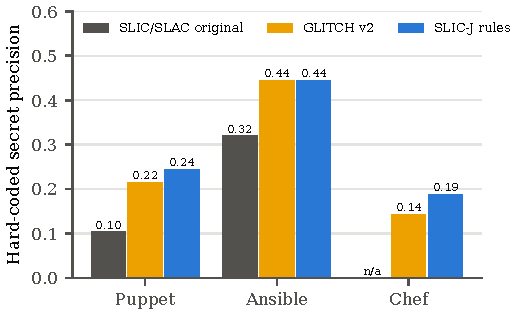
\includegraphics[width=\columnwidth]{figures/fig_secret.pdf}
\caption{Hard-coded secret precision on the oracles. Every rule-based tool stays below 0.45. (SLAC's Chef output has
no line numbers and cannot be scored.)}\label{fig:secret}
\end{figure}

\begin{table}[t]\centering\caption{RQ2: prevalence of the seven smells and the new TLS smell in the GLITCH corpora (occurrences / density per KLOC / \% of scripts).}\label{tab:rq2}
\scriptsize\setlength{\tabcolsep}{1.6pt}\begin{tabular}{lrrr}\toprule
 & Puppet & Ansible & Chef \\
Scripts & 27,324 & 107,955 & 70,705 \\
KLOC & 1,040 & 5,142 & 6,062 \\ \midrule
Admin by default & 1,452 / 1.40 / 2.0 & 10,367 / 2.02 / 5.7 & 2,565 / 0.42 / 2.1 \\
Empty password & 746 / 0.72 / 1.6 & 590 / 0.11 / 0.4 & 99 / 0.02 / 0.1 \\
Hard-coded secret & 4,814 / 4.63 / 7.6 & 35,145 / 6.84 / 12.5 & 10,719 / 1.77 / 6.8 \\
Invalid IP address binding & 245 / 0.24 / 0.7 & 2,657 / 0.52 / 1.0 & 1,270 / 0.21 / 0.9 \\
Suspicious comment & 1,806 / 1.74 / 4.4 & 5,718 / 1.11 / 3.6 & 10,634 / 1.75 / 8.1 \\
Use of HTTP without TLS & 1,547 / 1.49 / 3.2 & 8,184 / 1.59 / 3.8 & 11,653 / 1.92 / 5.5 \\
Use of weak crypto. algo. & 149 / 0.14 / 0.4 & 234 / 0.05 / 0.2 & 409 / 0.07 / 0.4 \\
\textit{TLS verif.\ disabled (new)} & 31 / 0.03 / 0.1 & 2,048 / 0.40 / 1.0 & 64 / 0.01 / 0.1 \\
\midrule Any of seven (\% scripts) & 14.5 & 18.2 & 18.7 \\
\bottomrule\end{tabular}\end{table}

On the 206{,}000-script corpora (Table~\ref{tab:rq2}), 14.5--18.7\% of scripts contain at least one of the seven
smells, below SLAC's 25.3--29.6\%: our rules no longer count variable references and lookups as hard-coded. The new
TLS smell appears in 1.01\% of Ansible scripts (2{,}048 occurrences; 1{,}690 are \texttt{validate\_certs: no}) but in
only 0.07\% of Puppet and 0.08\% of Chef scripts. On a random sample of 60 TLS findings (40 Ansible, 10 Puppet, 10
Chef), 59 are true (precision 0.98); the one false alarm is a test that \emph{asserts}
\texttt{OPENSTACK\_SSL\_NO\_VERIFY = False}. Several true findings target \texttt{https://localhost}, the same context
argument that practitioners raised against HTTP findings.

\subsection{RQ3: Context-aware triage}
\begin{table*}[t]\centering\caption{RQ3: triage of the 269 SLIC-J candidates (151 TP, 118 FP; 176 oracle smells). Mean $\pm$ s.d.\ over 10 seeds of grouped 5-fold CV (threshold tuned in-fold). Recall counts all oracle smells, so the rules' ceiling is 0.858. AUC, Brier and ECE use the raw scores; cost is USD per 1{,}000 findings; latency is the median per call.}\label{tab:rq3}
\scriptsize\setlength{\tabcolsep}{4pt}\begin{tabular}{llcccccccc}\toprule
Type & Method & Precision & Recall & F1 & F1 @0.5 & AUC & ECE & \$/1k & Lat.\,(s) \\ \midrule
Rules & SLIC-J rules only & 0.561$\pm$0.000 & 0.858$\pm$0.000 & 0.679$\pm$0.000 & -- & -- & -- & 0 & -- \\
Rules & Practitioner-context filter & 0.562$\pm$0.000 & 0.744$\pm$0.000 & 0.641$\pm$0.000 & -- & -- & -- & 0 & -- \\
\midrule
Learned & LogReg (context features) & 0.747$\pm$0.008 & 0.721$\pm$0.018 & 0.734$\pm$0.008 & 0.716 & 0.843 & 0.107 & 0 & -- \\
\midrule
Decision model & Jev 1.13, line only & 0.761$\pm$0.013 & 0.782$\pm$0.009 & 0.771$\pm$0.009 & 0.775 & 0.826 & 0.099 & 0.023 & 0.59 \\
Decision model & \textbf{Jev 1.13, full context} & 0.782$\pm$0.010 & 0.812$\pm$0.006 & 0.797$\pm$0.006 & 0.766 & 0.808 & 0.152 & 0.035 & 0.57 \\
Decision model & Jev 1.13, full, no comments & 0.785$\pm$0.009 & 0.811$\pm$0.009 & 0.797$\pm$0.007 & 0.768 & 0.816 & 0.140 & 0.035 & 0.57 \\
Decision model & Jev 1.14, full context & 0.774$\pm$0.005 & 0.798$\pm$0.011 & 0.786$\pm$0.007 & 0.796 & 0.795 & 0.180 & 0.035 & 0.66 \\
Decision model & GPT-6 Luna Decisions & 0.787$\pm$0.004 & 0.812$\pm$0.000 & 0.799$\pm$0.002 & 0.719 & 0.851 & 0.159 & 0.060 & 0.76 \\
Decision model & Liquid d1-ultra & 0.813$\pm$0.002 & 0.783$\pm$0.003 & 0.797$\pm$0.002 & 0.742 & 0.865 & 0.192 & 0.024 & 0.81 \\
Decision model & Perplexity Decider v1.2 & 0.799$\pm$0.004 & 0.787$\pm$0.012 & 0.793$\pm$0.005 & 0.784 & 0.865 & 0.143 & 0.011 & 0.74 \\
Decision model & Inception Mercury-Decide & 0.750$\pm$0.006 & 0.806$\pm$0.004 & 0.777$\pm$0.004 & 0.752 & 0.856 & 0.185 & 0.011 & 0.79 \\
Decision model & Cloudflare Clef & 0.776$\pm$0.011 & 0.732$\pm$0.003 & 0.753$\pm$0.005 & 0.753 & 0.850 & 0.070 & 0.028 & 0.79 \\
Decision model & Microsoft Decision-1 & 0.582$\pm$0.006 & 0.773$\pm$0.031 & 0.664$\pm$0.015 & 0.637 & 0.664 & 0.176 & 0.020 & 0.76 \\
Decision model & Upstage Solar-Decide & 0.624$\pm$0.013 & 0.784$\pm$0.002 & 0.694$\pm$0.008 & 0.697 & 0.511 & 0.307 & 0.042 & 1.89 \\
\midrule
Chat LLM & Claude Haiku 5.5 (chat LLM) & 0.785$\pm$0.005 & 0.839$\pm$0.008 & 0.811$\pm$0.005 & 0.644 & 0.843 & 0.178 & 0.143 & 1.78 \\
Chat LLM & Claude Haiku 5.5 via CLI (RQ4 arm) & 0.814$\pm$0.006 & 0.805$\pm$0.006 & 0.809$\pm$0.005 & 0.641 & 0.834 & 0.214 & -- & -- \\
\midrule
Hybrid & Hybrid: LogReg + Jev full & 0.833$\pm$0.013 & 0.702$\pm$0.008 & 0.762$\pm$0.006 & 0.759 & 0.875 & 0.073 & -- & -- \\
\bottomrule\end{tabular}\end{table*}

\begin{figure}[t]\centering
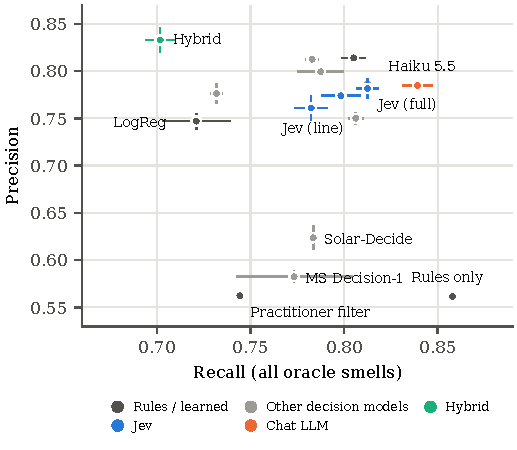
\includegraphics[width=\columnwidth]{figures/fig_pr.pdf}
\caption{Precision and recall of the triage methods (mean $\pm$ s.d.\ over 10 CV seeds). Triage moves the rules
(bottom right) up by 0.2 in precision for about 0.05 recall.}\label{fig:pr}
\end{figure}

\textbf{Triage works.} With the full state, Jev~1.13 raises precision from 0.561 to 0.782 and lowers recall from 0.858
to 0.812, so F1 rises from 0.679 to 0.797 (Table~\ref{tab:rq3}, Fig.~\ref{fig:pr}). The paired difference is
significant (McNemar: 80 candidates fixed vs.\ 9 broken, $p=2\times10^{-15}$; $\Delta$F1 $=+0.125$, 95\% CI
$[0.076, 0.179]$). Table~\ref{tab:rq3smell} shows where the gain comes from: for hard-coded secrets the false alarms fall
from 80 to 4 (precision 0.25$\to$0.83) while 7 of 27 true secrets are lost. Admin by default and IP binding, which are
already precise, are left untouched.

\begin{table}[t]\centering\caption{RQ3: per-smell precision / recall before and after triage (last CV seed). $n$ = oracle instances.}\label{tab:rq3smell}
\scriptsize\setlength{\tabcolsep}{3pt}\begin{tabular}{lrccc}\toprule
Smell & $n$ & Rules & Jev full & Hybrid \\ \midrule
Admin by default & 58 & 0.92/0.76 & 0.92/0.76 & 0.92/0.76 \\
Empty password & 10 & 0.86/0.60 & 0.83/0.50 & 0.86/0.60 \\
Hard-coded secret & 32 & 0.25/0.84 & 0.83/0.62 & 0.69/0.34 \\
Invalid IP address binding & 14 & 1.00/1.00 & 1.00/1.00 & 1.00/1.00 \\
Suspicious comment & 19 & 0.70/1.00 & 0.79/1.00 & 0.90/1.00 \\
Use of HTTP without TLS & 38 & 0.64/1.00 & 0.64/1.00 & 0.76/0.82 \\
Use of weak crypto. algo. & 5 & 0.43/0.60 & 0.40/0.40 & 0.50/0.20 \\
\bottomrule\end{tabular}\end{table}

\textbf{Context helps.} The full state beats the line-only state ($\Delta$F1 $=+0.028$, CI $[0.004, 0.053]$,
$p=0.013$). Jev also beats logistic regression on the same facts in paired decisions (33 vs.\ 15, $p=0.013$), but the
F1 interval includes zero ($[-0.008, 0.141]$). Removing comments from the state does not cost accuracy
(F1 0.797 both ways), which matters for RQ4.

\textbf{Practitioner context does not match the oracle.} The hand-written filter that encodes the practitioners'
objections from the original study lowers F1 to 0.641: the raters label placeholder passwords (\texttt{'password'},
\texttt{'ChangeThisPa55w0rd'}, \texttt{'vagrant'}) and templated \texttt{http://} URLs as smells. ``Is it a smell?''
and ``Should we fix it?'' are different questions, and an oracle answers only the first.

\textbf{Decision models differ.} Seven of the nine decision models land between F1 0.75 and 0.80;
GPT-6 Luna Decisions and Liquid d1-ultra tie with Jev~1.13, Jev~1.14 is slightly lower (0.786), and two models are
no better than the rules (Microsoft Decision-1, 0.664; Upstage Solar-Decide, 0.694, AUC 0.51). Pinning the model
version matters.

\textbf{Chat LLM vs.\ decision model.} Claude Haiku~5.5 reaches F1 0.811, but the paired difference to Jev is not
significant (11 vs.\ 6, $p=0.33$; CI $[-0.007, 0.048]$). Jev costs USD 0.035 per 1{,}000 findings at a median 0.57\,s
per call; Haiku costs USD 0.143 at 1.78\,s, i.e.\ $4.1\times$ the cost and $3.1\times$ the latency. Both are cheap in
absolute terms: triaging all 111{,}003 seven-sin findings of our corpora would cost about USD 3.9 with Jev and USD 15.9
with Haiku.

\begin{figure}[t]\centering
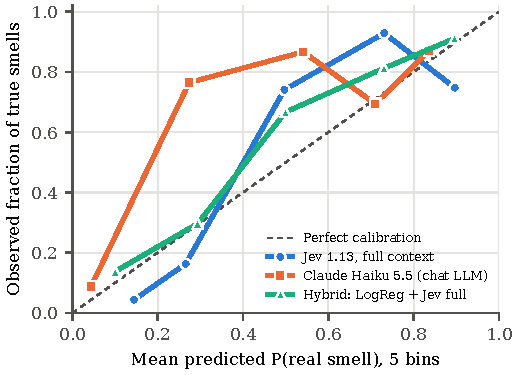
\includegraphics[width=\columnwidth]{figures/fig_reliability.pdf}
\caption{Reliability diagram. The raw probabilities of Jev and Haiku leave the diagonal (Haiku under-states the
share of true smells in the middle range); the hybrid, which lets code re-weight the model's answer with the context
facts, stays closest to it.}\label{fig:rel}
\end{figure}

\textbf{Calibration.} Raw probabilities are not calibrated (Jev ECE 0.152, Haiku 0.178; Fig.~\ref{fig:rel}): a
threshold of 0.5 is not a safe default for every model (e.g.\ Mercury-Decide's F1-optimal threshold is 0.05). The
hybrid has the best ranking and calibration of all methods (AUC 0.875, ECE 0.073) and the highest precision (0.833),
but its F1-tuned threshold trades away recall (0.702), so its F1 (0.762) is not better than Jev alone. A team that
wants to route uncertain findings to a human should use the hybrid's probabilities; a team that wants one keep/drop
decision should use the model with a tuned threshold.

\textbf{Errors.} The 9 true findings Jev dropped are mostly plain service user names (\texttt{nginx},
\texttt{zabbix}, \texttt{check}) and placeholder passwords (\texttt{foo}, \texttt{fixme}): cases the raters count as
smells by definition and a reviewer would call harmless. Most of the HTTP findings that the oracle marks false look
real (e.g.\ \texttt{http://download.sonatype.com/nexus/oss}), and Jev keeps them; we read these as missed oracle labels
rather than model errors.

\subsection{RQ4: Robustness to misleading comments}
\begin{table}[t]\centering\caption{RQ4: flip rate (true findings that the model drops after a misleading comment is inserted) with comments visible / removed from the state.}\label{tab:rq4}
\scriptsize\setlength{\tabcolsep}{3pt}\begin{tabular}{llcc}\toprule
Model & Attack (position) & Visible & Removed \\ \midrule
Claude Haiku 5.5 ($n$=59) & placeholder (above) & 16.4\% (9) & 0.0\% (0) \\
 & placeholder (inline) & 20.0\% (11) & 0.0\% (0) \\
 & approval (above) & 1.8\% (1) & 0.0\% (0) \\
 & approval (inline) & 1.8\% (1) & 0.0\% (0) \\
 & injection (above) & 0.0\% (0) & 0.0\% (0) \\
 & injection (inline) & 0.0\% (0) & 0.0\% (0) \\
\midrule
Mercury-Decide ($n$=132) & placeholder (above) & 26.2\% (32) & 1.6\% (2) \\
 & placeholder (inline) & 1.6\% (2) & 0.0\% (0) \\
 & approval (above) & 1.6\% (2) & 1.6\% (2) \\
 & approval (inline) & 1.6\% (2) & 0.0\% (0) \\
 & injection (above) & 97.5\% (119) & 1.6\% (2) \\
 & injection (inline) & 22.1\% (27) & 0.0\% (0) \\
\bottomrule\end{tabular}\end{table}

\begin{figure*}[t]\centering
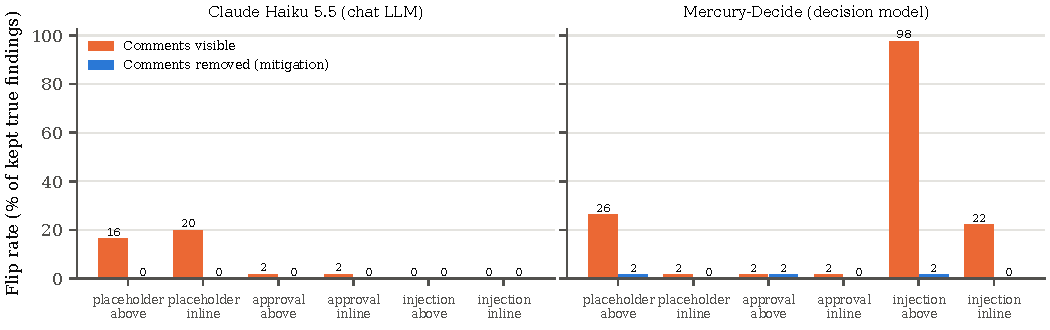
\includegraphics[width=\textwidth]{figures/fig_rq4.pdf}
\caption{RQ4: share of kept true findings that flip to ``drop'' after one inserted comment, with comments visible
(orange) and removed from the state (blue).}\label{fig:rq4}
\end{figure*}

One inserted comment is enough to defeat a decision model (Table~\ref{tab:rq4}, Fig.~\ref{fig:rq4}). For Mercury-Decide
the injection placed above the line flips 119 of 122 kept true findings (97.5\%) and the placeholder claim flips
26.2\%; the mean probability for true findings drops from 0.80 to 0.02 under injection. Inline variants are weaker
(22.1\% and 1.6\%). An authority claim (``approved by the security team'') has almost no effect (1.6\%).
The chat LLM behaves differently. Claude Haiku~5.5 ignores the explicit injection (0 of 55 flips) and the authority claim (1 of 55), but the \emph{placeholder} claim still flips 16.4\% (above) and 20.0\% (inline) of its kept true findings: the model does not obey the comment, it \emph{believes} it. A plausible statement of fact is the more dangerous attack for a model that resists instructions.

\textbf{Mitigation.} Removing comments from the state cuts every attack to at most 1.6\% for Mercury-Decide (the
same level as the noise from shifting a line number) and to 0\% for Haiku, and it costs no accuracy on clean data (RQ3). Our first version
stripped comments only from the code window and left them in the separate ``flagged line'' field: the inline injection
then still flipped 45.2\% of true findings. A mitigation has to cover every field the model can read.

% =====================================================================
\section{Discussion}
\textbf{For tool builders.} A linter that publishes rules should publish them as code, with tests built from the
paper's own examples: the printed admin rule fails on the paper's own Fig.~4, and the dead check would fail any
end-to-end test of its rule. Line numbers in outputs are not optional either: SLAC's Chef output carries none and cannot be
scored at line level.

\textbf{For SRE teams.} Keep rules as the high-recall front end; they are cheap, deterministic and explainable.
Put a decision model behind them only for the noisy smells (secrets, HTTP, comments), let code compute and mask
context, tune the threshold on your own labelled sample, and pin the model version. Never let script comments reach
the model: in a CI pipeline, the author of a pull request controls them.

\textbf{On ``context''.} Context improved precision only when it was given to a model that judged against the
\emph{definition}. Encoding the practitioners' notion of context as rules lowered F1 against the oracle. Future
evaluations should label two things per finding: whether it is a smell, and whether it is worth fixing in that
repository's context.

% =====================================================================
\section{Threats to Validity}
\textbf{Construct.} The oracles are small (43--79 scored smells per technology, 176 in total) and contain label noise
(Section~V-C); per-smell values for rare smells (weak crypto, empty password) rest on fewer than ten instances. TLS
precision was judged by one rater (the authors) on 60 findings; the labelled sheet is in the artifact for a second rater.

\textbf{Internal.} Rule refinement looked at the 30\% development split of the same oracles that we later use in
cross-validation; the triage thresholds never see test folds, but the candidate generator is not fully independent of
them. The Claude Code CLI loads the user's global instructions, so the RQ4 Haiku arm ran with a fixed but non-empty
context; it is the same for clean and attacked inputs.

\textbf{External.} RQ4 used a free decision model and a sample for Haiku because the API budget ran out; Jev's own
robustness is untested. All scripts are open source and pre-2022; private infrastructure code may differ.

\textbf{Reliability.} Hosted models change; we pin versions (e.g.\ \texttt{typesafe/jev-1.13-20260917}) and cache every
request and response, so all numbers can be regenerated without new API calls.

% =====================================================================
\section{Conclusion}
We reproduced SLIC, showed that its paper and its code disagree in six places, and built a Python port that matches
the original tool. Our port to Ansible and Chef is competitive with GLITCH and finds a new, common and precise smell:
disabled TLS verification in 1\% of Ansible scripts. Adding a context-aware decision model behind the rules raised
precision from 0.56 to 0.78 and F1 from 0.68 to 0.80, removed 95\% of the false hard-coded-secret alarms, and cost a few
cents per thousand findings. The same models can be told to ignore a true finding by a single comment, so the
comment text must stay out of their input. Rules propose, a model disposes, and code stays in charge.

\section*{Artifact}
The repository contains the \texttt{slicj} package (parsers, rules, context, triage), tests built from the paper's
Figs.~4--5, the experiment scripts for RQ1--RQ4, the cached model responses, and a README that regenerates every table
and figure.

\bibliographystyle{IEEEtran}
\bibliography{references}
\end{document}
